\documentclass[conference]{IEEEtran}
\IEEEoverridecommandlockouts

\usepackage{cite}
\usepackage{amsmath,amssymb}
\usepackage{graphicx}
\usepackage{booktabs}
\usepackage{url}
\usepackage{xcolor}
\usepackage{listings}
\usepackage{tikz}
\DeclareUnicodeCharacter{2212}{\ensuremath{-}}
\usetikzlibrary{positioning,arrows.meta,fit}

\lstset{
  language=Python,
  basicstyle=\ttfamily\scriptsize,
  keywordstyle=\color{blue!60!black},
  commentstyle=\color{gray},
  stringstyle=\color{red!50!black},
  columns=fullflexible,
  breaklines=true,
  frame=single,
  framerule=0.3pt,
  showstringspaces=false
}

% Figures are read from the repository's figures/ folder.
\graphicspath{{../}}

\begin{document}

\title{Remaining Useful Life Prediction of Lithium-Ion Cells under Varying Usage Conditions with LSTM, Attention and Swish\\
\large MASC 520 Final Project}

\author{\IEEEauthorblockN{Junbo Shim}
\IEEEauthorblockA{\textit{Mork Family Department of Chemical Engineering and Materials Science}\\
\textit{University of Southern California}, Los Angeles, CA, USA\\
junboshi@usc.edu}}

\maketitle

\begin{abstract}
Battery lifetime depends on usage, so a lifetime model must generalize to usage conditions not seen in training. This study predicts the remaining useful life (RUL) of 245 lithium-polymer cells from the ISU-ILCC dataset, cycled under 63 combinations of charge rate, discharge rate and depth of discharge, and tests every model only on held-out conditions. An LSTM with causal self-attention and a Swish output head achieved a mean absolute error (MAE) of 147.4 equivalent full cycles (EFC), 27\% lower than that of a random forest using only the usage conditions (203.0~EFC) but higher than that of one using the same inputs (137.7~EFC). The three LSTM variants had MAEs within 2.0~EFC of one another. In the first 20\% of life, the mean lifetime of other cells tested under the same condition predicted RUL more accurately than any fitted model, and models using the capacity history surpassed this benchmark only after about 40\% of life. Split-conformal calibration on held-out training groups raised the coverage of a quantile LSTM's 10--90\% interval from 73\% to 76\%, short of the nominal 80\%.
\end{abstract}

\begin{IEEEkeywords}
lithium-ion battery, remaining useful life, LSTM, attention, Swish, deep learning
\end{IEEEkeywords}

%=====================================================================
\section{Introduction}
%=====================================================================
\subsection{Why remaining useful life matters}
\label{sec:why}
Lithium-ion batteries lose capacity with every charge and discharge, and their end of life is commonly defined as a fraction of the original capacity, for example 80\% for smartphone and laptop batteries \cite{apple} and about 70\% under typical electric-vehicle (EV) battery warranties \cite{npr2026}. The remaining useful life (RUL) is the amount of use left before this threshold; this study uses the common laboratory threshold of 80\% of rated capacity. Accurate RUL prediction supports replacement decisions by device owners, warranty design by manufacturers and the valuation of retired EV batteries for second-life use, where cells with the same capacity can have very different remaining lives \cite{gu2024}.

\subsection{Why usage makes RUL hard to predict}
The rate of capacity fade depends on usage. Temperature, state of charge and current all affect the rate of aging \cite{woody2020}. In a multi-year study at Sandia National Laboratories, cells of the same chemistry cycled within the manufacturer's specifications reached 80\% capacity thousands of hours and cycles apart, depending on the cycling conditions \cite{preger2020}.

The dataset used in this study shows the same effect (Fig.~\ref{fig:overview}). Cells cycled at 20--40\% depth of discharge had a median lifetime of 1,373 equivalent full cycles, compared with 545 for cells cycled beyond 80\%. Lifetimes also varied among cells cycled under identical conditions: within the median experimental group, the longest-lived cell lasted 1.5 times as long as the shortest-lived one, and up to 3.1 times as long within a single group. An RUL model must therefore account for usage and generalize to usage patterns absent from the training data, since no test campaign can cover every way batteries are used in practice.

\subsection{Research question and contributions}
Long short-term memory (LSTM) networks \cite{hochreiter1997} are widely used for RUL prediction because capacity measurements form a time series \cite{liu2017,zraibi2025}. Most such studies, however, use the NASA or CALCE datasets, in which all cells share one or a few test conditions \cite{chen2023,tran2025}, so a model can perform well simply by recognizing the condition. This study investigates whether an LSTM outperforms simpler models given the same information when the test cells come from usage conditions absent from training, and whether attention and the Swish activation improve its accuracy.

The main contributions of this study are as follows:
\begin{enumerate}
\item A per-test RUL dataset of 3,956 capacity tests of 245 cells, constructed from the raw ISU-ILCC records.
\item An LSTM with causal self-attention and a Swish output head, compared with two random forests, one with identical inputs.
\item An evaluation on unseen usage conditions, in which entire experimental groups are held out.
\item Diagnostics of the error: a same-condition benchmark, a feature ablation of the forest, and split-conformal 10--90\% intervals.
\end{enumerate}

%=====================================================================
\section{Related Work}
%=====================================================================
LSTMs have been applied to the CALCE \cite{liu2017} and NASA \cite{zraibi2025} datasets, and later studies add an attention mechanism (CA-LSTM) \cite{chen2023} or combine 1-D convolution with attentional and ODE-based LSTMs \cite{tran2025}.

Another line of work predicts lifetime from features measured early in life. Severson \emph{et al.} predicted cycle life from how the discharge voltage curve changed over the first 100 cycles \cite{severson2019}. Li \emph{et al.} created the ISU-ILCC dataset used here, deliberately varying the charge rate, discharge rate and depth of discharge, and used it to predict lifetime under varying usage from early aging data \cite{li2024,thelen2023}.

The model in this study follows the common LSTM approach and adds the attention mechanism of \cite{vaswani2017} and the Swish activation of \cite{ramachandran2017}. It differs from prior work mainly in its evaluation, which uses unseen usage conditions and baselines that receive identical inputs.

%=====================================================================
\section{Data and Assumptions}
\label{sec:data}
%=====================================================================
\subsection{Cells and test conditions}
The ISU-ILCC battery aging dataset \cite{thelen2023} was collected by Iowa State University (ISU) and Iowa Lakes Community College (ILCC) to study how charge rate, discharge rate and depth of discharge (DoD) affect capacity fade.
\begin{itemize}
\item \textbf{Cells:} 251 commercial 502030 lithium-polymer pouch cells (Shenzhen Honghaosheng Electronics), NMC cathode, graphite anode, 250~mAh rated capacity, 3.0--4.2~V.
\item \textbf{Equipment:} two 64-channel Neware BTS-4000 cyclers, one at each site, with the cells in incubators at 30~$^\circ$C.
\item \textbf{Cycling:} a constant-current, constant-voltage (CC-CV) charge, then a constant-current discharge that stops at a voltage cutoff chosen to give the group's DoD.
\item \textbf{Reference performance tests (RPTs):} after every 7 days of cycling, one full cycle at C/5 and one at C/2; this study uses the C/5 discharge capacity. Groups 20--64 had an additional RPT after the first 3.5 days, and groups 30--64 had pulse tests for internal resistance, which were not used. Testing stopped below 80\% capacity.
\end{itemize}

Each of the 63 experimental groups has its own charge rate, discharge rate and DoD (Fig.~\ref{fig:overview}a). In groups 1--25 the discharge rate was kept near 0.5C while the charge rate (0.5--3C) and the DoD were varied; groups 26--64 varied all three factors over the full range. Table~\ref{tab:data} summarizes the cells used in this study, and Fig.~\ref{fig:fade} in the appendix shows the capacity fade of each cell.

\begin{table}[t]
\centering
\caption{Dataset used in this study}
\label{tab:data}
\begin{tabular}{@{}ll@{}}
\toprule
Cells / experimental groups & 245 / 63 \\
Cell type & 502030 pouch, NMC/graphite \\
Rated capacity, temperature & 250~mAh, 30~$^\circ$C \\
Capacity tests (rows) & 3,956 \\
Tests per cell, median (range) & 14 (2--59) \\
Total life, EFC, median (range) & 784 (85--1,939) \\
Charge rate & 0.50--3.01C \\
Discharge rate & 0.49--2.48C \\
Depth of discharge & 3.5--99.5\% \\
Initial capacity, mean & 113.4\% of rated \\
\bottomrule
\end{tabular}
\end{table}

\begin{figure*}[t]
\centering
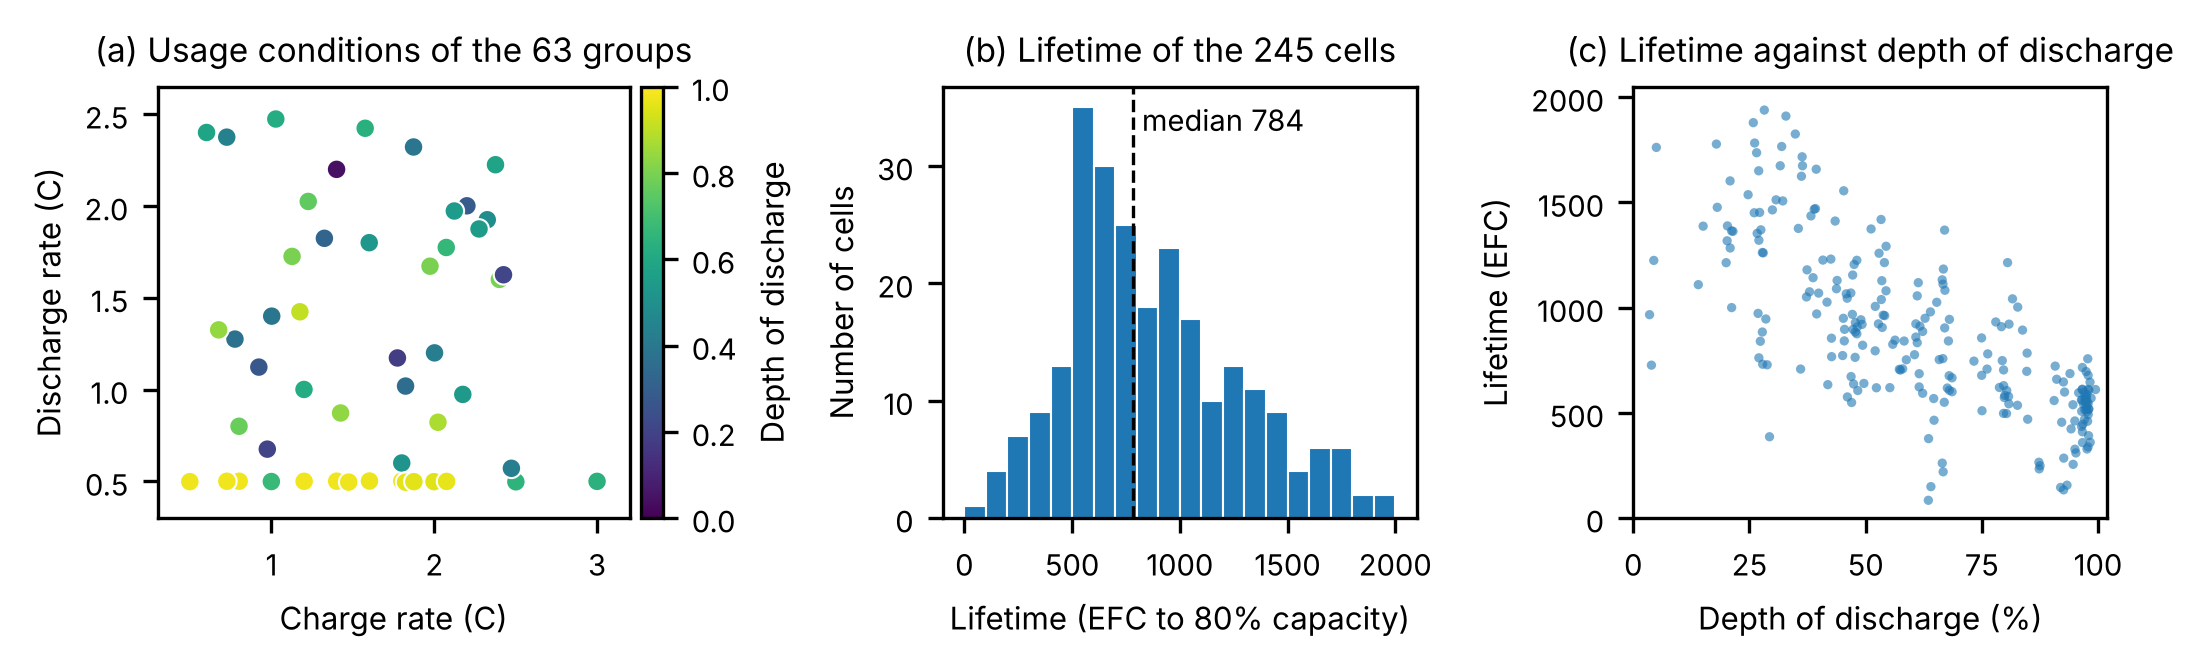
\includegraphics[width=\textwidth]{figures/dataset_overview.png}
\caption{(a) Charge rate, discharge rate and depth of discharge of the 63 experimental groups. (b) Lifetime of the 245 cells, in equivalent full cycles until the capacity fell to 80\% of rated. (c) Lifetime against depth of discharge. The vertical spread at a given DoD includes cells of the same group, which were cycled under identical conditions.}
\label{fig:overview}
\end{figure*}

\subsection{Raw data processing}
The dataset stores two JSON files per cell, about 11~GB in total, named by the cell ID (G36C4 is cell 4 of group 36). The RPT file holds, for every RPT, the C/5 and C/2 capacities, the voltage, current and charge traces, and the start and stop times; the cycling file holds the same for every regular cycle. The processed capacity-fade curves in the release are indexed by time on test, whereas usage in equivalent full cycles requires the capacity of every cycle, so the raw files were processed in Google Colab into a 0.5~MB table with one row per RPT (Table~\ref{tab:columns}). Six cells that never reached 80\% capacity or had incomplete records were excluded. Among the cycles with a recorded start time, no discharge capacity was missing, so no values had to be filled. Five cycles without a start time were excluded from the EFC count (effect at most 0.6~EFC).

\begin{table}[t]
\centering
\caption{How each column of the table is computed}
\label{tab:columns}
\footnotesize
\setlength{\tabcolsep}{3pt}
\begin{tabular}{@{}p{1.55cm}p{6.85cm}@{}}
\toprule
Column & Source and computation \\
\midrule
capacity & RPT file: C/5 discharge capacity at every RPT before EOL \\
efc\_so\_far & Cycling file: capacity discharged in all cycles that started before the RPT, summed and divided by 0.25~Ah \\
rul\_efc & From capacity and efc\_so\_far, with EOL interpolated at 200~mAh (Section~\ref{sec:labels}) \\
c\_chg & Cycling file: maximum current of each of the first 30 charges, median over cycles, divided by 0.25~A \\
c\_dis & Cycling file: median current of each of the first 30 discharges, median over cycles, divided by 0.25~A \\
dod & Cycling file: median discharged capacity of the first 10 cycles divided by the first RPT capacity \\
\bottomrule
\end{tabular}
\end{table}

The usage conditions were computed from the current records rather than taken from the documentation, so that the same procedure applies to cells without documented conditions; Section~\ref{sec:formulation} compares the two.

\subsection{Labels}
\label{sec:labels}
A cycle does not represent the same amount of use across conditions: a cell cycled at 4\% DoD ran more than 60,000 cycles, whereas one at 97\% ran a few hundred. Usage is therefore measured in \emph{equivalent full cycles} (EFC): the cumulative discharged capacity divided by the rated capacity $Q_r = 0.25$~Ah,
\begin{equation}
\mathrm{EFC}_k = \frac{1}{Q_r}\sum_{j \in \mathcal{C}_k} q_j ,
\end{equation}
where $\mathcal{C}_k$ is the set of cycles that started before test $k$ and $q_j$ is the capacity discharged in cycle $j$. If test $k$ is the first with capacity $C_k$ below $0.8\,Q_r = 0.2$~Ah, the end of life (EOL) lies between tests $k-1$ and $k$ and is obtained by linear interpolation:
\begin{equation}
\mathrm{EFC}_{\mathrm{EOL}} = \mathrm{EFC}_{k-1} + \frac{C_{k-1} - 0.2}{C_{k-1} - C_k}\left(\mathrm{EFC}_k - \mathrm{EFC}_{k-1}\right),
\end{equation}
The label at every earlier test is then $\mathrm{RUL}_k = \mathrm{EFC}_{\mathrm{EOL}} - \mathrm{EFC}_k$.

\emph{Worked example.} Table~\ref{tab:example} in the appendix lists the seven tests of cell G36C4 before its end of life, interpolated at 284.9~EFC between its seventh and eighth tests; each RUL is 284.9~EFC minus the EFC used up to that test, and the seven rows form one input sequence.

\begin{figure*}[t]
\centering
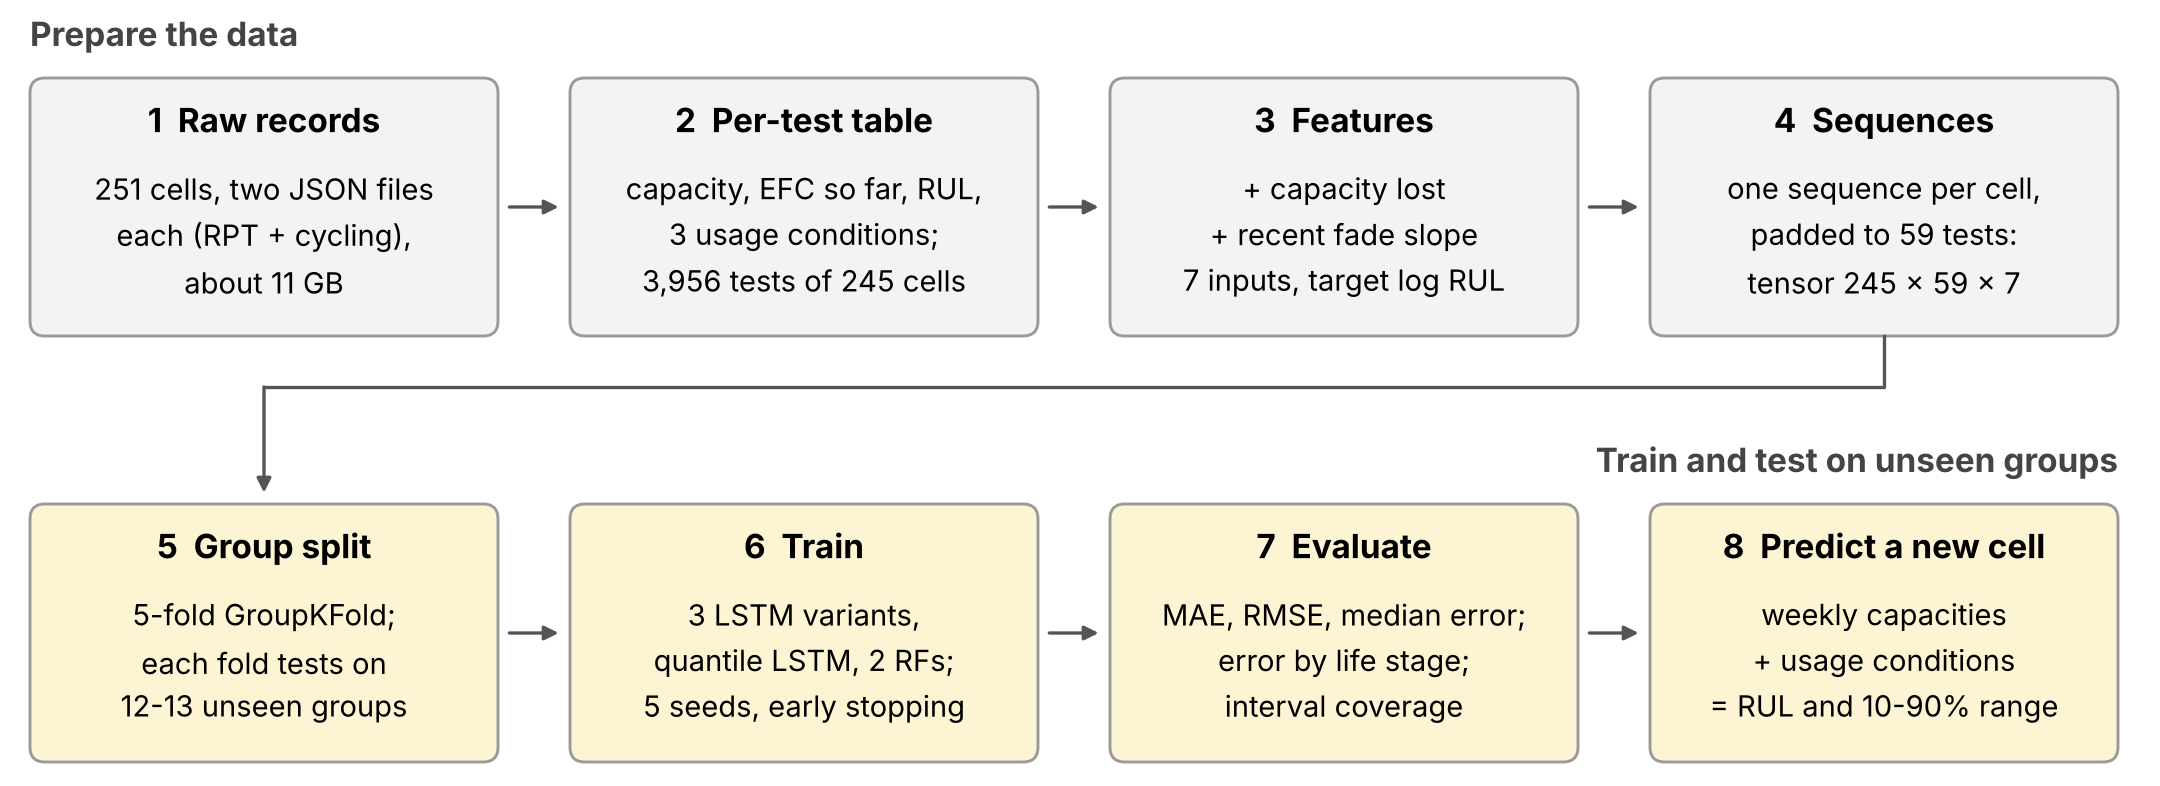
\includegraphics[width=0.94\textwidth]{figures/pipeline.png}
\caption{Workflow of this study. Gray: data preparation. Yellow: training and testing on experimental groups excluded from training.}
\label{fig:pipeline}
\end{figure*}

\subsection{Assumptions}
The results rest on three assumptions. First, each cell's usage protocol is known before testing and remains constant. In practice, the charge delivered per cycle decreases with aging because discharge terminates at a fixed voltage (G1C1: 0.070~Ah in its first cycle and 0.048~Ah at the median); the initial DoD is therefore used, as it is the value known in advance. Second, cells within a group are interchangeable, which is why test cells are always drawn from groups absent from training. Third, EFC is an adequate measure of life; because the cells were cycled continuously, calendar aging is not captured.

%=====================================================================
\section{Methodology}
%=====================================================================
\subsection{Pipeline overview}
Fig.~\ref{fig:pipeline} summarizes the workflow; steps 1--2 are implemented in the notebook \texttt{01\_build\_dataset} and steps 3--8 in \texttt{02\_train\_models}. Step 3 adds the capacity lost and fade slope, standardizes the seven inputs with the fitting cells of each fold, and takes $\log$ RUL as the target. In step 4 each cell becomes one sequence, padded to 59 tests with a mask that excludes padded steps from the loss, the attention and the metrics. Steps 5--7 split the data by group, train every deep model with five seeds and score each prediction, which at test $k$ uses only tests 1 to $k$ (Sections~\ref{sec:formulation}--\ref{sec:eval}); step 8 retrains on all cells to predict a new cell.

\subsection{Problem formulation}
\label{sec:formulation}
For cell $i$ with tests $k = 1, \dots, T_i$, the model receives the sequence $\mathbf{x}_{i,1}, \dots, \mathbf{x}_{i,k}$ and predicts $\mathrm{RUL}_{i,k}$. Each test has seven inputs: the measured capacity $C_k$, $\mathrm{EFC}_k$, the capacity lost so far $C_1 - C_k$, the recent fade slope
\begin{equation}
s_k = \frac{C_k - C_{k-2}}{\mathrm{EFC}_k - \mathrm{EFC}_{k-2}} \quad (s_1 = s_2 = 0),
\end{equation}
and the three usage conditions. Inputs are standardized with training statistics. RUL ranges over more than an order of magnitude, so the target is $y_k = \log \max(\mathrm{RUL}_k, 10)$. The floor of 10 keeps the last test before EOL from dominating the loss.

\emph{Information at each prediction.} At test $k$ the model uses the capacities and EFC of tests 1 to $k$ and the three usage conditions. The conditions are computed from the cell's first 30 cycles (rates) and first 10 cycles (DoD), which run after the first capacity test, so the results assume that the cycling protocol is known before the test starts. In this dataset each group follows a protocol set in advance: the computed rates match the documented protocol \cite{thelen2023} within 0.01C for every cell, and the computed DoD is within 3 percentage points of its group's documented mean DoD for 90\% of cells. If the conditions had to be measured on the cell itself, the first valid prediction would come after 30 cycles: at the second test for 84\% of cells and at the third for the rest. Appendix~\ref{app:training} reports the errors on these 3,671 tests.

\subsection{Model and training}
Fig.~\ref{fig:model} shows the model. An LSTM with 32 hidden units processes the tests in order, so its state $\mathbf{h}_k$ depends only on tests up to $k$. A single-head self-attention layer \cite{vaswani2017} then allows each step to attend to all earlier states:
\begin{align}
\alpha_{kj} &= \operatorname{softmax}_{j \le k}\!\left(\frac{(W_Q\mathbf{h}_k)^{\top} W_K\mathbf{h}_j}{\sqrt{d}}\right),\\
\mathbf{c}_k &= W_O \sum_{j \le k} \alpha_{kj} W_V \mathbf{h}_j .
\end{align}
A causal mask enforces $j \le k$, so no prediction uses future tests. The output head maps the combined state to the log RUL,
\begin{equation}
\hat{y}_k = \mathbf{w}_2^{\top}\,\mathrm{swish}\!\left(W_1[\mathbf{h}_k;\mathbf{c}_k] + \mathbf{b}_1\right) + b_2,
\end{equation}
with $\mathrm{swish}(z) = z\,\sigma(z)$ \cite{ramachandran2017}. Unlike ReLU, Swish is smooth and passes small negative values (Fig.~\ref{fig:swish}). The full model has 11,585 trainable parameters, and 6,337 without attention.

\begin{figure}[t]
\centering
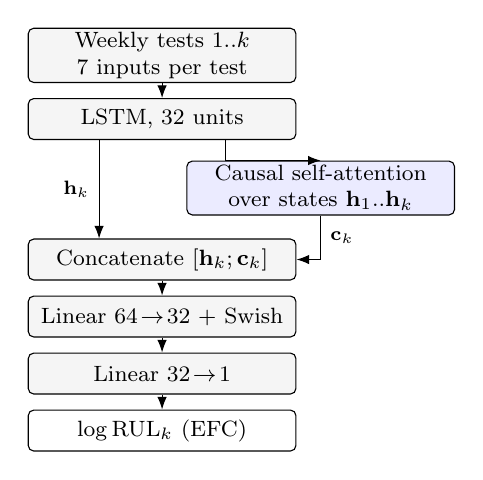
\begin{tikzpicture}[
  node distance=1.9mm,
  blk/.style={draw, rounded corners=2pt, align=center, font=\footnotesize, minimum width=34mm, minimum height=5.2mm, inner sep=1.5pt, fill=gray!8},
  att/.style={blk, fill=blue!8},
  arr/.style={-{Latex[length=1.6mm]}, thin}]
\node[blk] (in) {Weekly tests $1..k$\\ 7 inputs per test};
\node[blk, below=of in] (lstm) {LSTM, 32 units};
\node[att, below right=2.6mm and -14mm of lstm] (att) {Causal self-attention\\ over states $\mathbf{h}_1..\mathbf{h}_k$};
\node[blk, below=12.5mm of lstm] (cat) {Concatenate $[\mathbf{h}_k;\mathbf{c}_k]$};
\node[blk, below=of cat] (fc1) {Linear $64\!\to\!32$ + Swish};
\node[blk, below=of fc1] (fc2) {Linear $32\!\to\!1$};
\node[blk, below=of fc2, fill=white] (out) {$\log \mathrm{RUL}_k$ (EFC)};
\draw[arr] (in) -- (lstm);
\draw[arr] (lstm.south) ++(-8mm,0) -- ([xshift=-8mm]cat.north) node[midway, left, font=\scriptsize] {$\mathbf{h}_k$};
\draw[arr] (lstm.south) ++(8mm,0) |- ([yshift=0mm]att.north) ;
\draw[arr] (att.south) |- ([yshift=0mm]cat.east) node[pos=0.25, right, font=\scriptsize] {$\mathbf{c}_k$};
\draw[arr] (cat) -- (fc1);
\draw[arr] (fc1) -- (fc2);
\draw[arr] (fc2) -- (out);
\end{tikzpicture}
\caption{Model. The ``LSTM + Swish'' variant omits the attention branch, and the ``attention + ReLU'' variant replaces Swish with ReLU.}
\label{fig:model}
\end{figure}

The loss is the mean squared error of $\hat{y}_k$ over the real (unpadded) steps. The model is trained with Adam \cite{kingma2015} at a learning rate of $3\times10^{-3}$ with weight decay $10^{-4}$ and mini-batches of 32 cells, and the output bias is initialized to the mean target. Training uses early stopping: 20\% of the training groups are held out, the validation MAE is checked every two epochs, and training stops after 20 epochs without improvement (120 at most), keeping the best weights. The training procedure was chosen by comparing configurations on the test folds (Appendix~\ref{app:training}).

\subsection{Prediction intervals}
A point prediction conveys no information about its uncertainty. Two methods of attaching an interval to each prediction were compared:
\begin{itemize}
\item \textbf{Spread of training runs}: the interval between the lowest and highest predictions of the five LSTM runs.
\item \textbf{Quantile LSTM}: the same network with three outputs instead of one, trained to predict the 10th, 50th and 90th percentiles $\hat{y}^{(\tau)}$ of the log RUL with the pinball loss
\begin{equation}
L_\tau = \max\!\left(\tau\,(y - \hat{y}^{(\tau)}),\ (\tau - 1)\,(y - \hat{y}^{(\tau)})\right),
\end{equation}
$\tau \in \{0.1, 0.5, 0.9\}$.
\end{itemize}
For $\tau = 0.9$, under-prediction is penalized nine times more heavily than over-prediction, which drives that output toward the 90th percentile. A well-calibrated 10--90\% interval therefore contains the true RUL 80\% of the time. Training, early stopping and folds are the same as for the other deep models, and the five runs' percentiles are averaged. The share of held-out tests whose true RUL falls inside an interval is its \emph{coverage}.

\textbf{Split-conformal calibration.} The quantile interval is widened in log space to $[\hat{y}^{(0.1)}-c,\ \hat{y}^{(0.9)}+c]$ by conformalized quantile regression \cite{romano2019}. Inside each fold, 20\% of the training groups are set aside; the quantile LSTM is trained on the rest, and $c$ is the 80th percentile of the scores $\max(\hat{y}^{(0.1)}-y,\ y-\hat{y}^{(0.9)})$ on the set-aside groups, per bin of the predicted share of life used, $\mathrm{EFC}_k/(\mathrm{EFC}_k+\hat{r}^{(0.5)}_k)$. The held-out fold is used only for the final evaluation.

\subsection{Evaluation and baselines}
\label{sec:eval}
All models are evaluated with five-fold \texttt{GroupKFold} by experimental group, so every prediction is for a condition the model was not trained on. Each deep model is trained five times from different random seeds. Performance is reported as MAE and root mean squared error (RMSE) in EFC, and as the median relative error $|\hat{r}-r|/r$. Because cells have 2 to 59 tests, the MAE weights long-lived cells more; the cell-averaged MAE, the mean of each cell's MAE, weights every cell equally. The ensemble MAE is the error of the average of the five runs' predictions. The error is also broken down by the share of life already used, $\mathrm{EFC}_k / \mathrm{EFC}_{\mathrm{EOL}}$. Three deep variants are compared: LSTM + Swish (no attention), LSTM + attention + ReLU, and LSTM + attention + Swish.

Two random forests \cite{breiman2001} (300 trees, at least two samples per leaf) are trained on the same folds:
\begin{itemize}
\item \textbf{Conditions only} predicts the log total life from the three usage conditions. The RUL is the predicted total minus $\mathrm{EFC}_k$. This model does not use any capacity measurement of the cell.
\item \textbf{Fade features} receives the same seven inputs as the deep models at each test, but not the sequence; the capacity lost and fade slope provide a summary of the history.
\end{itemize}
Further analyses put the errors in context. A \textbf{same-condition benchmark} predicts each held-out cell from the mean life of the other cells of its group, information that no deployed model has. A \textbf{feature ablation} adds the inputs of the fade-feature forest to the usage conditions one at a time. A \textbf{learning curve} retrains the LSTM + attention + Swish and the fade-feature forest on 20--100\% of each fold's training groups (five random subsets per size).


%=====================================================================
\section{Results}
\label{sec:results}
%=====================================================================
\subsection{Model comparison}
Table~\ref{tab:results} summarizes the results. The largest improvement comes from giving a model access to the capacity history: the error falls from 203.0~EFC for the conditions-only forest to 137.7--149.4~EFC for the other models. Among the seven-input models, the random forest on fade features is the most accurate single model. The best deep model, LSTM + attention + Swish, achieves an MAE of 147.4~EFC, or 140.4~EFC when the predictions of its five runs are averaged.

\begin{table}[t]
\centering
\caption{RUL prediction error on unseen experimental groups (EFC)}
\label{tab:results}
\setlength{\tabcolsep}{4pt}
\newcommand{\hd}[1]{\begin{tabular}[b]{@{}r@{}}#1\end{tabular}}
\begin{tabular}{@{}lrrrrrr@{}}
\toprule
Model & MAE & \hd{Seed\\std} & \hd{Ens.\\MAE} & \hd{Cell\\MAE} & RMSE & \hd{Med.\\err.} \\
\midrule
RF, conditions only & 203.0 & -- & -- & 178.1 & 270.6 & 40.1\% \\
RF, fade features & \textbf{137.7} & -- & -- & \textbf{120.7} & \textbf{211.8} & \textbf{22.7\%} \\
LSTM + Swish & 149.4 & 3.7 & 142.6 & 129.2 & 227.4 & 25.5\% \\
LSTM + att.\ + ReLU & 147.8 & 5.4 & 140.7 & 129.0 & 225.8 & 24.8\% \\
LSTM + att.\ + Swish & 147.4 & 4.6 & 140.4 & 130.2 & 220.8 & 25.5\% \\
\bottomrule
\end{tabular}
\\[2pt]
\footnotesize Deep models: mean over five runs; Ens.\ = average of the five runs' predictions; Cell MAE = mean of each cell's MAE.
\end{table}

The MAEs of the three deep variants are within 2.0~EFC of one another, whereas the MAE of the same model trained from different random seeds has a standard deviation of 3.7--5.4~EFC. With five runs per variant, the experiment therefore cannot rank the variants. Fig.~\ref{fig:pred} in the appendix plots the predicted against the true RUL for the best model, and Fig.~\ref{fig:cells} shows the predictions for four held-out cells over their lifetimes. Weighting every cell equally (cell MAE) lowers all errors; the fade-feature forest remains the most accurate (120.7~EFC, against 123.1--124.3~EFC for the LSTM ensembles), but the order of the three LSTM variants changes, as expected for differences within seed variation. The feature ablation shows where the forest's advantage comes from. Adding the EFC used to the usage conditions did not help (204.7~EFC), but adding the current capacity reduced the MAE to 155.3~EFC, about three quarters of the gain to 137.7~EFC. Adding capacity lost (148.4~EFC), fade slope (143.3~EFC) or both (137.7~EFC) supplied the rest, with the largest relative gain in the last 20\% of life (46.3 to 32.4~EFC); no input set improved the first 20\% (218--226~EFC). In the learning curve (Fig.~\ref{fig:lc}), the MAE of the LSTM fell from 194.6 to 147.4~EFC and that of the forest from 166.8 to 137.7~EFC as the training groups per fold grew from 10 to 50, so the gap narrowed from 28 to 10~EFC. Changes to the training procedure mattered more than the architecture (Appendix~\ref{app:training}).

\subsection{Error over the life of a cell}
Fig.~\ref{fig:life} breaks the error down by the share of life already used. In the first 20\%, all models have errors of 218--226~EFC, and the capacity history provides no advantage over the usage conditions alone. Thereafter, the error of the models that use the history decreases steadily, to 32--40~EFC in the last 20\% of life, whereas the conditions-only forest remains at about 211--237~EFC until the final stage and a straight-line extrapolation of the capacity trend errs by 86~EFC even in the last 20\% (Appendix~\ref{app:training}).

\begin{figure}[t]
\centering
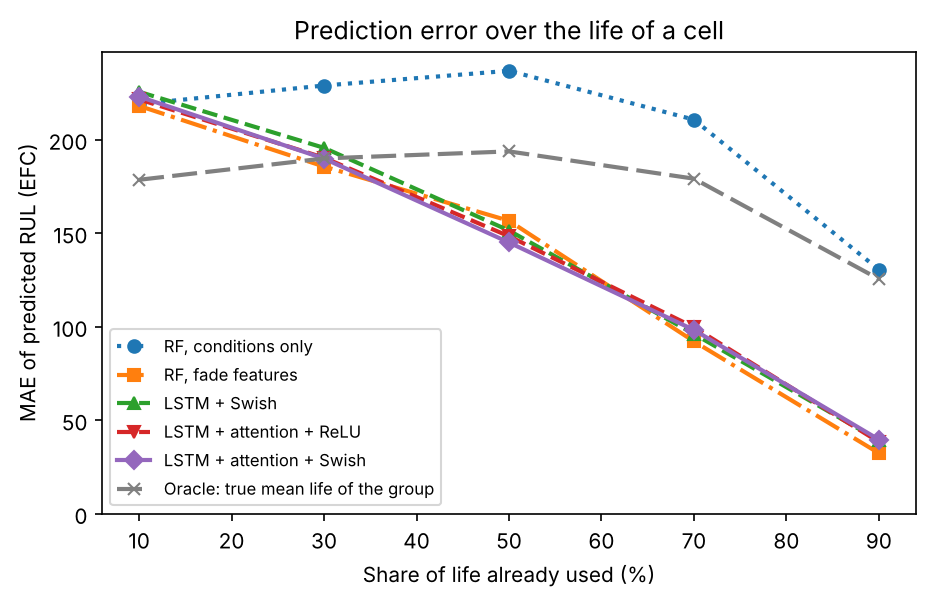
\includegraphics[width=\columnwidth]{figures/error_over_life.png}
\caption{MAE of predicted RUL by the share of life already used. Deep models are shown as five-run ensembles; the gray line is the same-condition benchmark (mean life of the other cells in the group).}
\label{fig:life}
\end{figure}

\subsection{A same-condition benchmark}
\label{sec:sources}
On the 3,923 tests whose group has another cell, the same-condition benchmark has an MAE of 171.7~EFC, between the conditions-only forest (202.9~EFC) and the fade-feature forest (138.0~EFC). In the first 20\% of life, however, it was more accurate than any fitted model (179 vs.\ 219--223~EFC); the models that use the capacity history matched it at 20--40\% of life and surpassed it only after about 40\% (Fig.~\ref{fig:life}). Its error combines the spread between identically cycled cells with the error of estimating a group mean from about three cells, so it is a reference point, not a lower bound. Adding three $\Delta Q(V)$ summaries of the weekly voltage curve (Appendix~\ref{app:curve}) lowered the forest's MAE from 137.7 to 132.2~EFC; in the first 20\% of life it fell only from 218.0 to 214.9~EFC, a change within the uncertainty of the estimate.

\subsection{Prediction intervals}
\label{sec:resintervals}
Table~\ref{tab:intervals} compares the interval methods. The spread of training runs contains the true RUL only 33\% of the time: the five runs agree with one another far more closely than with the observed values. The quantile LSTM's 10--90\% interval contains it 73\% of the time, short of the nominal 80\%, and its coverage is lowest in the last 20\% of life (68.8\%), where the interval is narrowest. There, 21\% of true RULs fell below the interval and 10\% above it; 6.7\% of these tests had a true RUL below the 10~EFC floor of the training target, and flooring them would raise the coverage to 71.7\%. For split-conformal calibration, a quantile LSTM trained on 80\% of each fold's training groups had a raw coverage of 73.2\% and a median width of 386~EFC; calibration on the remaining groups raised the coverage to 76.2\% (71.8\% in the last 20\% of life), still short of 80\%, and the median width by 15\%, to 444~EFC. Coverage was uneven across groups (median 83\%, below 50\% for 8 of the 63 groups). The quantile median has an MAE of 141.5~EFC, close to the point model's five-run ensemble (140.4~EFC).

\begin{table}[t]
\centering
\caption{Coverage (\%) and median width (EFC) of the prediction intervals on held-out groups}
\label{tab:intervals}
\setlength{\tabcolsep}{3pt}
\begin{tabular}{@{}lrrrrrr@{}}
\toprule
 & \multicolumn{2}{c}{Run spread} & \multicolumn{2}{c}{Quantile} & \multicolumn{2}{c}{Conformal} \\
\cmidrule(lr){2-3}\cmidrule(lr){4-5}\cmidrule(l){6-7}
Life used & Cov. & Width & Cov. & Width & Cov. & Width \\
\midrule
All & 32.6 & 106 & 73.2 & 362 & 76.2 & 444 \\
0--20\% & 27.6 & 151 & 76.4 & 665 & 78.2 & 720 \\
20--40\% & 31.3 & 152 & 74.4 & 493 & 79.1 & 599 \\
40--60\% & 34.6 & 134 & 72.6 & 371 & 76.3 & 476 \\
60--80\% & 33.6 & 98 & 73.5 & 253 & 75.7 & 303 \\
80--100\% & 37.1 & 37 & 68.8 & 88 & 71.8 & 101 \\
\bottomrule
\end{tabular}
\\[2pt]
\footnotesize Conformal: quantile LSTM refit on 80\% of each fold's training groups and calibrated on the other 20\% (before calibration: 73.2\% coverage, 386~EFC width).
\end{table}

Fig.~\ref{fig:intervals} in the appendix shows the intervals for the four held-out cells of Fig.~\ref{fig:cells}; only for G63C4, which outlived its group, does the true RUL lie mostly outside the interval.


%=====================================================================
\section{Observations and Discussion}
%=====================================================================
The same-condition benchmark gives the most informative result: in the first 20\% of life, the lifetimes of sibling cells predicted RUL better than any model that observed the cell's own capacity. Cells cycled identically age differently, and early in life this does not show in the capacity, which falls slowly at first and drops sharply after a knee (Fig.~\ref{fig:fade}). Knees can arise from lithium plating, electrode saturation, resistance growth or electrolyte depletion, some of which build up with little electrochemical signature beforehand \cite{attia2022}. G63C4 (Fig.~\ref{fig:cells}) is an example: neither its usage nor its early capacity distinguished it from its group, and all models predicted half to two-thirds of its true RUL early in life.

The data show associations, not their causes; known degradation mechanisms of NMC/graphite cells suggest possible explanations. Depth of discharge was most strongly associated with lifetime (Spearman $\rho = -0.76$ across cells). Deeper cycles strain the active particles more, which can crack them and expose fresh surface to SEI growth, so that lithium inventory and active material are lost faster \cite{woody2020}. Among cells cycled above 80\% DoD, higher charge rate was associated with shorter life ($\rho = -0.30$, $p = 0.01$); lithium plating on graphite at high charging currents, a common cause of knees, is one possible explanation \cite{attia2022}. Faster discharge was associated with longer life in EFC ($\rho = +0.39$), which may reflect calendar aging, since slowly cycled cells spend more time per EFC at 30~$^\circ$C, or the design of the test matrix. Near the end of life, the models overestimated RUL (Section~\ref{sec:resintervals}), consistent with fade accelerating after a knee. The voltage-curve features (Appendix~\ref{app:curve}) reduced the error most at 20--60\% of life, possibly because the discharge curve changes measurably only once degradation has progressed.

The ablation explains much of the forest's strength: most of its gain over the conditions-only model comes from the current capacity. Both models received this and the other fade summaries directly, and with these inputs the LSTM did not achieve a lower MAE than the forest. The learning curve is consistent with a data limitation (245 sequences with a median of 14 tests), since the LSTM gained more than the forest from added groups; both were still improving at about 50 groups, so whether the LSTM would overtake the forest remains open. With sequences this short, attention may add little to the LSTM state.

Split-conformal calibration improved the coverage of the quantile interval but left it below the nominal level, likely because ten calibration groups per fold do not represent every held-out condition. In practice (Section~\ref{sec:why}), a warranty set before any fade is observed faces the conditions-only error of 203.0~EFC, about a quarter of the median lifetime of 784~EFC.

This study has several limitations. The training procedure was chosen on the same folds that produce the reported errors (Appendix~\ref{app:training}), so the deep-model errors are likely optimistic by an unmeasured amount; the forests were not tuned, so this bias favors the LSTM and the forest's lead is, if anything, understated. The first prediction of each cell assumes that its usage protocol is known in advance (Section~\ref{sec:formulation}). All cells were small 250~mAh cells cycled at 30~$^\circ$C with constant currents, so the model remains unverified for other temperatures, dynamic loads and discharge rates below 0.49C.

%=====================================================================
\section{Conclusion}
%=====================================================================
This study evaluated RUL prediction for lithium-ion cells on usage conditions excluded from training. The capacity history reduced the MAE from 203.0~EFC to 137.7--149.4~EFC, in the forest mostly through the current capacity, but the LSTM with attention and Swish did not outperform a random forest given the same inputs, and the effects of attention and Swish were within seed-to-seed variation. In the first 20\% of life, the mean lifetime of sibling cells predicted RUL better than any fitted model. Split-conformal calibration raised the coverage of the quantile intervals from 73\% to 76\%, short of the nominal 80\%. Three $\Delta Q(V)$ summaries of the weekly voltage curve lowered the forest's MAE to 132.2~EFC but its first-20\% error only from 218.0 to 214.9~EFC, so earlier signs of cell-to-cell differences are still needed. Code and data are available at \url{https://github.com/junbo9/battery-rul-lstm-attention}.

%=====================================================================
\begin{thebibliography}{00}
\bibitem{apple} Apple Inc., ``Battery service and recycling.'' [Online]. Available: \url{https://www.apple.com/batteries/service-and-recycling/} (accessed Nov. 2026).
\bibitem{npr2026} NPR, ``How long do electric vehicle batteries actually last?,'' Mar.~2, 2026. [Online]. Available: \url{https://www.npr.org/2026/03/02/nx-s1-5706658/electric-vehicle-battery-lifespan}
\bibitem{gu2024} X. Gu \emph{et al.}, ``Challenges and opportunities for second-life batteries: Key technologies and economy,'' \emph{Renewable and Sustainable Energy Reviews}, vol.~192, 2024, arXiv:2308.06786.
\bibitem{woody2020} M. Woody, M. Arbabzadeh, G. M. Lewis, G. A. Keoleian, and A. Stefanopoulou, ``Strategies to limit degradation and maximize Li-ion battery service lifetime -- Critical review and guidance for stakeholders,'' \emph{Journal of Energy Storage}, vol.~28, Art.~no.~101231, 2020.
\bibitem{preger2020} Y. Preger \emph{et al.}, ``Degradation of commercial lithium-ion cells as a function of chemistry and cycling conditions,'' \emph{Journal of The Electrochemical Society}, vol.~167, no.~12, Art.~no.~120532, 2020.
\bibitem{hochreiter1997} S. Hochreiter and J. Schmidhuber, ``Long short-term memory,'' \emph{Neural Computation}, vol.~9, no.~8, pp.~1735--1780, 1997.
\bibitem{liu2017} Y. Liu, G. Zhao, X. Peng, and C. Hu, ``Lithium-ion battery remaining useful life prediction with long short-term memory recurrent neural network,'' in \emph{Proc. Annu. Conf. PHM Society}, vol.~9, no.~1, 2017, doi: 10.36001/phmconf.2017.v9i1.2447.
\bibitem{zraibi2025} B. Zraibi and M. Mansouri, ``Improving lithium-ion battery reliability through neural network remaining useful life prediction,'' \emph{IAES Int. J. Artif. Intell.}, vol.~14, no.~1, pp.~83--91, 2025, doi: 10.11591/ijai.v14.i1.pp83-91.
\bibitem{chen2023} C. Chen, J. Wei, and Z. Li, ``Remaining useful life prediction for lithium-ion batteries based on a hybrid deep learning model,'' \emph{Processes}, vol.~11, no.~8, Art.~no.~2333, 2023, doi: 10.3390/pr11082333.
\bibitem{tran2025} K. Tran, T. Le, B. Huynh, H.-C. Trinh, and V.-R. Nguyen, ``End-to-end framework for predicting the remaining useful life of lithium-ion batteries,'' arXiv:2505.16664, 2025.
\bibitem{severson2019} K. A. Severson \emph{et al.}, ``Data-driven prediction of battery cycle life before capacity degradation,'' \emph{Nature Energy}, vol.~4, pp.~383--391, 2019.
\bibitem{li2024} T. Li, Z. Zhou, A. Thelen, D. Howey, and C. Hu, ``Predicting battery lifetime under varying usage conditions from early aging data,'' \emph{Cell Reports Physical Science}, 2024, arXiv:2307.08382.
\bibitem{thelen2023} A. Thelen, T. Li, J. Liu, C. Tischer, and C. Hu, ``ISU-ILCC battery aging dataset,'' Iowa State University, 2023, doi: 10.25380/iastate.22582234.
\bibitem{vaswani2017} A. Vaswani \emph{et al.}, ``Attention is all you need,'' in \emph{Advances in Neural Information Processing Systems}, vol.~30, 2017.
\bibitem{ramachandran2017} P. Ramachandran, B. Zoph, and Q. V. Le, ``Searching for activation functions,'' arXiv:1710.05941, 2017.
\bibitem{kingma2015} D. P. Kingma and J. Ba, ``Adam: A method for stochastic optimization,'' in \emph{Proc. Int. Conf. Learning Representations (ICLR)}, 2015.
\bibitem{romano2019} Y. Romano, E. Patterson, and E. J. Cand\`es, ``Conformalized quantile regression,'' in \emph{Advances in Neural Information Processing Systems 32 (NeurIPS)}, 2019, pp.~3543--3553.
\bibitem{breiman2001} L. Breiman, ``Random forests,'' \emph{Machine Learning}, vol.~45, no.~1, pp.~5--32, 2001.
\bibitem{attia2022} P. M. Attia \emph{et al.}, ``Review---`Knees' in lithium-ion battery aging trajectories,'' \emph{Journal of The Electrochemical Society}, vol.~169, no.~6, Art.~no.~060517, 2022.
\end{thebibliography}

%=====================================================================
\clearpage
\onecolumn
\appendices
\section{Additional Figures and Tables}

\begin{table}[h]
\centering
\caption{The seven capacity tests of cell G36C4}
\label{tab:example}
\footnotesize
\setlength{\tabcolsep}{4pt}
\begin{tabular}{@{}rrrrrr@{}}
\toprule
Test & Capacity & EFC & Cap.\ lost & Slope & RUL \\
 & (mAh) & so far & (mAh) & (mAh/100 EFC) & (EFC) \\
\midrule
1 & 283.3 & 0.0 & 0.0 & 0.0 & 284.9 \\
2 & 242.5 & 27.1 & 40.8 & 0.0 & 257.9 \\
3 & 236.9 & 55.4 & 46.4 & $-83.7$ & 229.5 \\
4 & 233.2 & 112.1 & 50.1 & $-10.9$ & 172.8 \\
5 & 230.6 & 168.2 & 52.7 & $-5.6$ & 116.8 \\
6 & 223.6 & 222.9 & 59.7 & $-8.7$ & 62.0 \\
7 & 205.6 & 275.2 & 77.7 & $-23.4$ & 9.7 \\
\bottomrule
\end{tabular}
\end{table}

\begin{figure}[h]
\centering
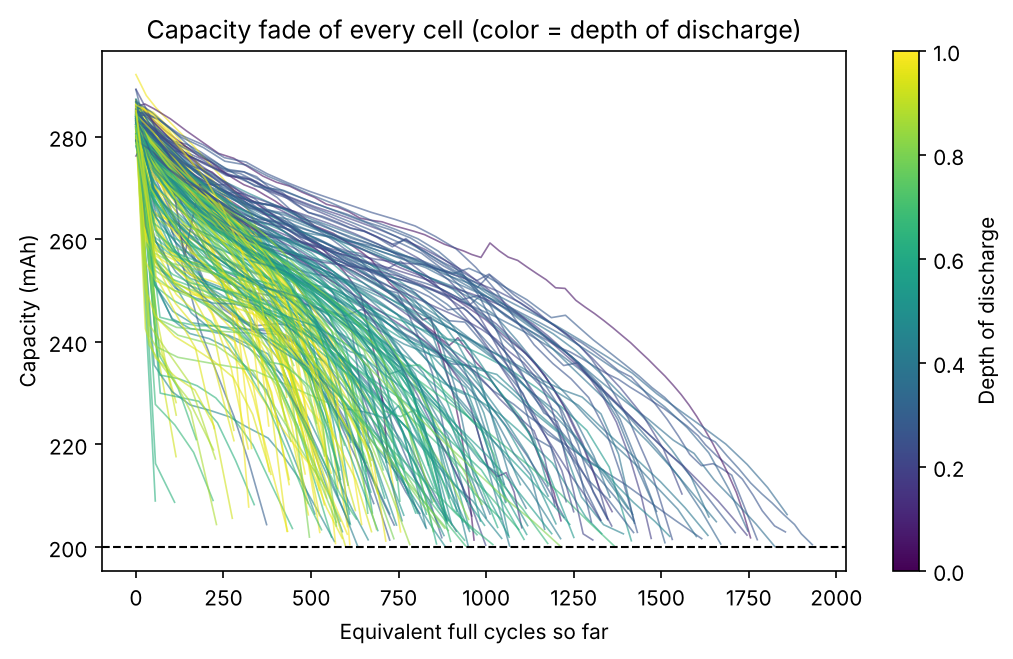
\includegraphics[width=0.62\textwidth]{figures/capacity_fade.png}
\caption{Capacity against equivalent full cycles for every cell, colored by depth of discharge. The dashed line marks the end of life (200~mAh).}
\label{fig:fade}
\end{figure}

\begin{figure}[h]
\centering
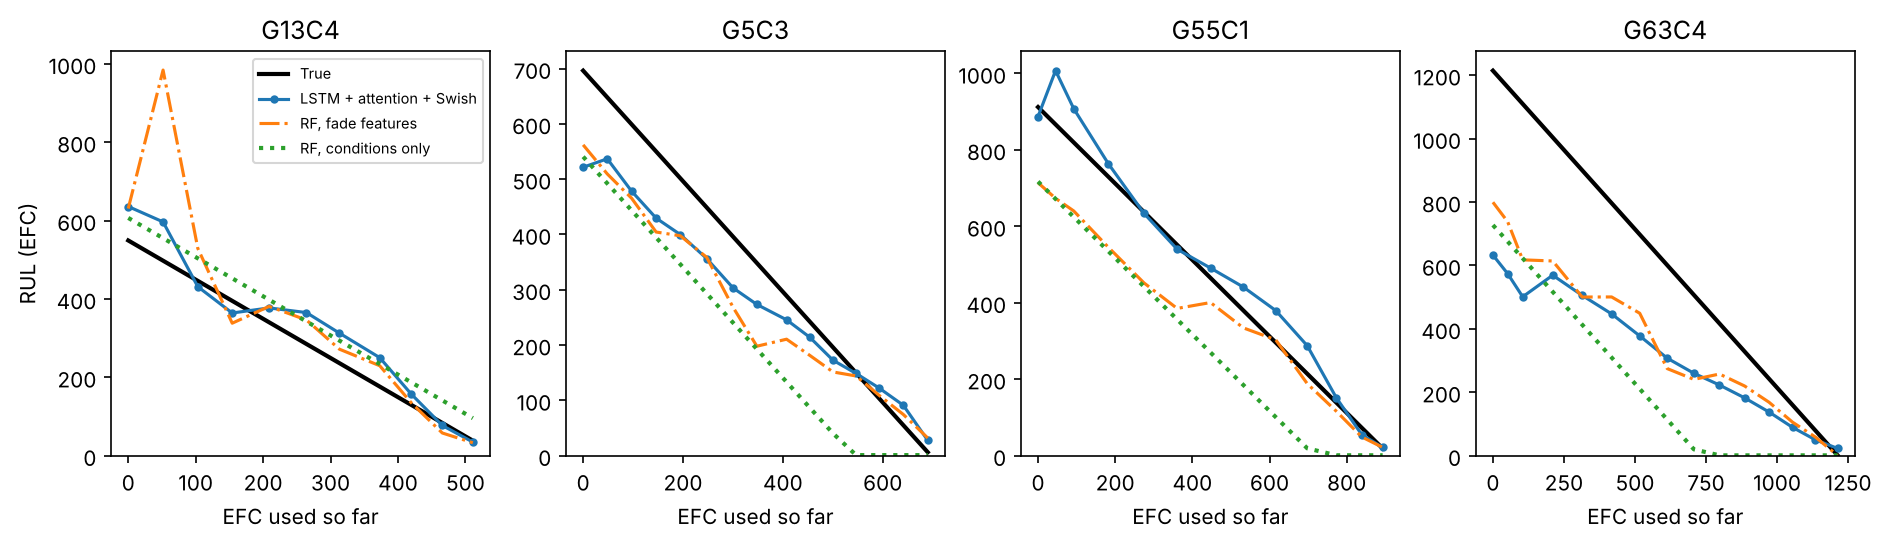
\includegraphics[width=\textwidth]{figures/example_cells.png}
\caption{True and predicted RUL over the life of four held-out cells, chosen across the range of lifetimes.}
\label{fig:cells}
\end{figure}

\begin{figure}[h]
\centering
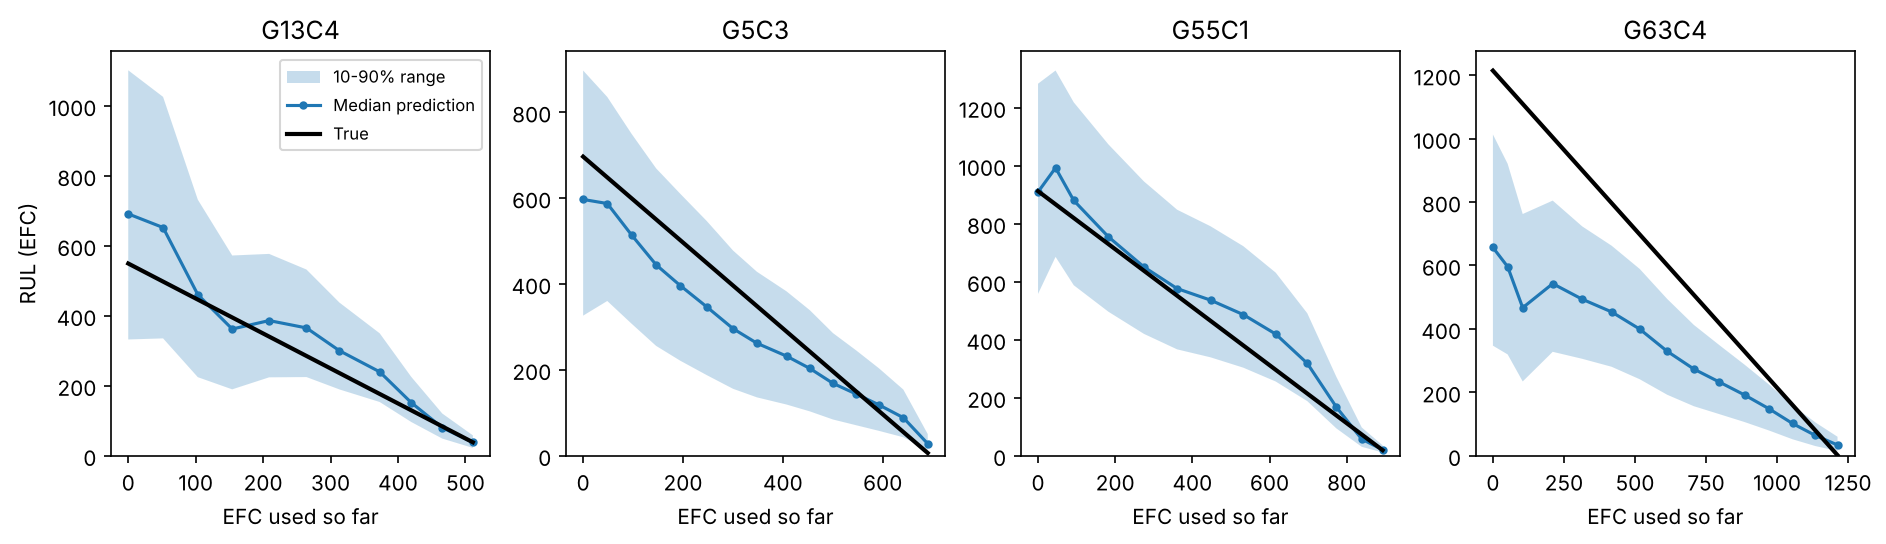
\includegraphics[width=\textwidth]{figures/prediction_intervals.png}
\caption{Median prediction and 10--90\% prediction interval of the quantile LSTM for four held-out cells.}
\label{fig:intervals}
\end{figure}

\begin{figure}[h]
\centering
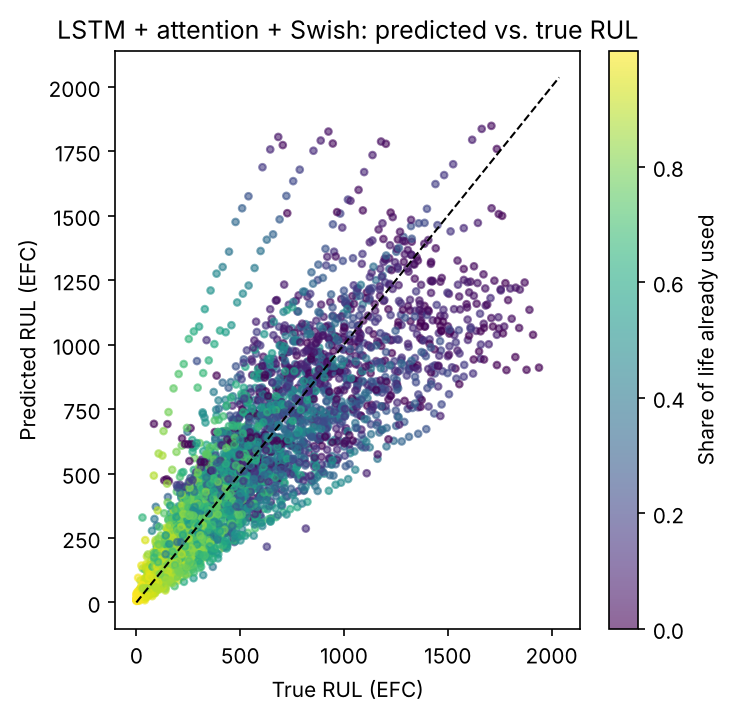
\includegraphics[width=0.5\textwidth]{figures/predicted_vs_true.png}
\caption{Predicted against true RUL for the LSTM + attention + Swish ensemble on held-out groups. Color shows the share of life already used.}
\label{fig:pred}
\end{figure}

\begin{figure}[h]
\centering
\begin{minipage}[t]{0.55\textwidth}
\centering
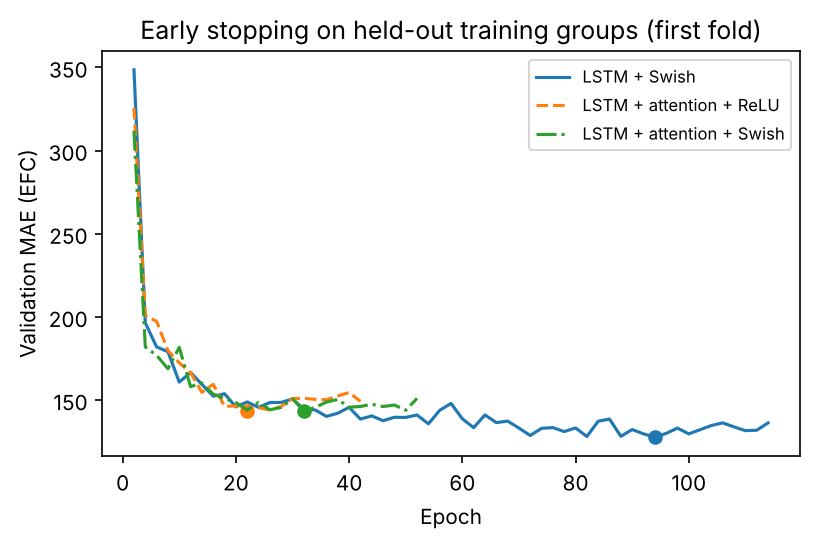
\includegraphics[width=\textwidth]{figures/early_stopping.png}
\caption{Validation MAE on the held-out training groups of the first fold during training. Dots mark the epochs kept by early stopping.}
\label{fig:es}
\end{minipage}\hfill
\begin{minipage}[t]{0.42\textwidth}
\centering
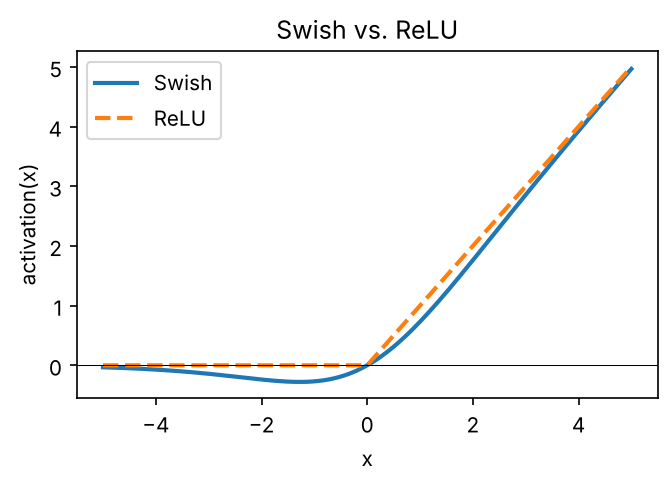
\includegraphics[width=\textwidth]{figures/swish_vs_relu.png}
\caption{The Swish and ReLU activation functions.}
\label{fig:swish}
\end{minipage}
\end{figure}

\begin{figure}[h]
\centering
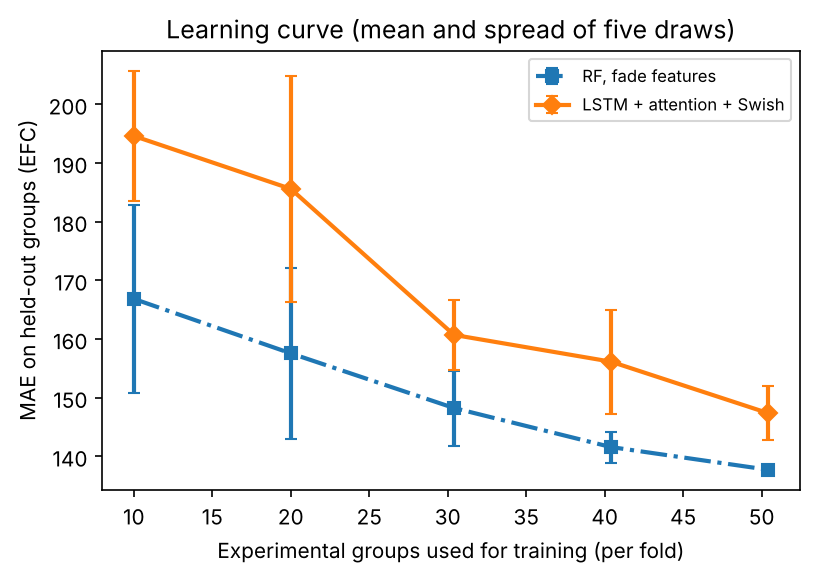
\includegraphics[width=0.6\textwidth]{figures/learning_curve.png}
\caption{Learning curve: MAE on held-out groups against the number of training groups per fold (mean and standard deviation over five random subsets).}
\label{fig:lc}
\end{figure}

\clearpage
\section{Voltage-Curve Features}
\label{app:curve}
For every weekly test, the C/5 discharge curve was interpolated to the discharged capacity $Q(V)$ on 400 voltages between 3.40 and 4.05~V, the range covered by every curve. The change since the first test, $\Delta Q(V) = Q_k(V) - Q_0(V)$, was summarized by its mean, minimum and log variance, as in \cite{severson2019}. Four further features were the C/2-to-C/5 capacity ratio, the voltage and height of the largest $dQ/dV$ peak, and the capacity discharged down to 3.40~V. One of the 3,956 tests had no usable curve and kept the values of the previous test. The fade-feature forest and the LSTM + attention + Swish were retrained with these inputs on the same folds (Table~\ref{tab:curve}).

Adding the three $\Delta Q(V)$ summaries reduced the forest's MAE from 137.7 to 132.2~EFC. In a bootstrap over the 63 groups, the change was −5.5~EFC (95\% interval −10.2 to −1.0~EFC), and 40 of the 63 groups improved; most of the gain came at 20--60\% of life (−13.6~EFC). In the first 20\% of life, the change was −3.1~EFC (95\% interval −8.6 to +3.4~EFC), and the forest (214.9~EFC) stayed well behind the same-condition benchmark (178.5~EFC). The four other curve features added little. For the LSTM, adding $\Delta Q(V)$ changed the MAE from 147.4 to 145.5~EFC, within the seed-to-seed spread. Within groups, the mean of $\Delta Q(V)$ in weeks 2--4 had Spearman correlations of 0.22--0.28 with total life, compared with 0.08--0.17 for the capacity.

\begin{table}[h]
\centering
\caption{Error with features of the voltage curve (MAE in EFC, same folds)}
\label{tab:curve}
\footnotesize
\begin{tabular}{@{}lrrrrrrr@{}}
\toprule
Model & MAE & Cell MAE & 0--20\% & 20--40\% & 40--60\% & 60--80\% & 80--100\% \\
\midrule
RF, seven inputs & 137.7 & 120.7 & 218.0 & 185.6 & 156.6 & 92.1 & 32.4 \\
RF + $\Delta Q(V)$ & 132.2 & 116.1 & 214.9 & 174.7 & 140.4 & 90.0 & 34.2 \\
RF + all curve features & 132.0 & 115.3 & 212.2 & 176.9 & 142.6 & 89.0 & 33.7 \\
LSTM + att.\ + Swish & 147.4 & 130.2 & 230.9 & 199.3 & 154.1 & 104.8 & 42.2 \\
LSTM + att.\ + Swish + $\Delta Q(V)$ & 145.5 & 129.1 & 224.5 & 195.0 & 155.6 & 102.1 & 45.6 \\
LSTM + att.\ + Swish, ensemble & 140.4 & 124.3 & 223.0 & 189.8 & 145.0 & 98.2 & 39.6 \\
LSTM + att.\ + Swish + $\Delta Q(V)$, ensemble & 138.6 & 123.3 & 216.2 & 186.6 & 147.3 & 95.1 & 42.5 \\
\bottomrule
\end{tabular}
\\[2pt]
Percentage columns: share of life already used. Deep models: mean over five runs, or their ensemble. Same-condition benchmark in the first 20\% of life: 178.5~EFC.
\end{table}

\clearpage
\section{Training Procedure and Additional Analyses}
\label{app:training}
The training procedure was selected by comparing the MAE of 16 configurations on the five test folds. They varied the output floor and bias initialization, the number of epochs, the learning rate and its schedule, full-batch versus mini-batch training, early stopping, the input set, a linear target with the Huber loss, dropout, attention and the activation. The layer sizes (32 hidden LSTM units, one attention head and a 32-unit head) and the forest settings (300 trees, at least two samples per leaf) were fixed beforehand and not tuned. Changes to the training procedure and inputs affected accuracy more than the architecture did. The first version (LSTM + Swish, five inputs, full-batch training for 300 epochs) had an MAE of 159.1~EFC; training for 800 epochs with a higher learning rate ($10^{-2}$) and a cosine schedule raised it to 199.3~EFC, as the model fitted the training conditions more closely but generalized worse. Mini-batch training, early stopping on held-out groups (Fig.~\ref{fig:es}) and two additional inputs (capacity lost and fade slope) reduced the error of the same architecture to 149.4~EFC, an improvement of 9.7~EFC, larger than any difference among the variants.

The straight-line baseline extends the capacity trend through the last two tests to 200~mAh without any training. Until the capacity starts to fall it uses the conditions-only forest, and its predictions are capped at the largest RUL in the training folds. Its MAE was 396.5~EFC overall and 86.0~EFC in the last 20\% of life, against 32.4 and 39.6~EFC for the fade-feature forest and the LSTM ensemble.

The held-out conditions were rarely extrapolations: only 8 of the 63 groups lay outside the training range in any condition, and a group's relative error was not correlated with the distance from its condition to the nearest training condition (Spearman $\rho$ = 0.06--0.20, $p \ge 0.12$). In terms of the number of tests, the median error of the LSTM fell below 15\% of a cell's total life only after about six weekly tests. On the 3,671 tests after the first 30 cycles, where measured conditions would be available (Section~\ref{sec:formulation}), the conditions-only forest, the LSTM + attention + Swish and the fade-feature forest had MAEs of 204.3, 142.9 and 133.9~EFC (135.8~EFC for the LSTM ensemble), the same order as on all tests.

\clearpage
\section{Code}
All code is available in the repository: \texttt{01\_build\_dataset.ipynb} builds the dataset from the raw records, and \texttt{02\_train\_models.ipynb} trains and evaluates all models. The excerpts below show the model and the training loop.

\subsection{Model}
\begin{lstlisting}
class RULNet(nn.Module):
    def __init__(self, n_features, hidden=32, attention=True, activation='swish'):
        super().__init__()
        act = nn.SiLU() if activation == 'swish' else nn.ReLU()            # nn.SiLU is Swish
        self.lstm = nn.LSTM(n_features, hidden, batch_first=True)
        self.attention = nn.MultiheadAttention(hidden, num_heads=1, batch_first=True) if attention else None
        self.head = nn.Sequential(nn.Linear(hidden * (2 if attention else 1), 32), act, nn.Linear(32, 1))

    def forward(self, x, padding, return_weights=False):
        states, _ = self.lstm(x)                                           # (cells, steps, hidden)
        weights = None
        if self.attention is not None:
            t = x.shape[1]
            future = torch.triu(torch.ones(t, t, dtype=torch.bool, device=x.device), diagonal=1)
            context, weights = self.attention(states, states, states, attn_mask=future, key_padding_mask=padding)
            states = torch.cat([states, context], dim=-1)                  # current state + attended history
        out = self.head(states).squeeze(-1)                                # log(RUL) at every step
        return (out, weights) if return_weights else out
\end{lstlisting}

\subsection{Training with early stopping (one fold)}
\begin{lstlisting}
BATCH, LR, MAX_EPOCHS, PATIENCE, CHECK_EVERY = 32, 3e-3, 120, 20, 2

model = RULNet(len(FEATURES), attention=attention, activation=activation)
with torch.no_grad():
    model.head[-1].bias.fill_(float(Y[fit][M[fit]].mean()))         # start at the mean target
optimizer = torch.optim.Adam(model.parameters(), lr=LR, weight_decay=1e-4)

best_error, best_epoch, best_state = np.inf, 0, None
for epoch in range(1, MAX_EPOCHS + 1):
    model.train()
    order = torch.randperm(len(x))
    for start in range(0, len(x), BATCH):
        b = order[start:start + BATCH]
        optimizer.zero_grad()
        loss = ((model(x[b], ~m[b]) - y[b])[m[b]] ** 2).mean()         # padded steps are excluded
        loss.backward()
        optimizer.step()
    if epoch % CHECK_EVERY == 0:                                       # validate on held-out training groups
        model.eval()
        with torch.no_grad():
            pred_val = np.exp(model(x_val, pad_val).numpy())
        error = np.abs(pred_val - RUL[val])[M[val]].mean()
        if error < best_error:
            best_error, best_epoch = error, epoch
            best_state = {k: v.clone() for k, v in model.state_dict().items()}
        elif epoch - best_epoch >= PATIENCE:
            break
model.load_state_dict(best_state)
\end{lstlisting}

\subsection{Cross-validation by experimental group}
\begin{lstlisting}
cv = GroupKFold(n_splits=5)
FOLDS = list(cv.split(cell_ids, groups=cell_group))   # a group is never split between training and test
\end{lstlisting}

\end{document}
